\documentclass[compress,11pt]{beamer}
%\includeonly{pendel}
\usetheme{Ilmenau}
%\usetheme{fau-4-3}
%\usecolortheme{beaver}
\beamertemplatenavigationsymbolsempty
\usepackage[ngerman]{babel}
\usepackage{marvosym}
\usepackage{multimedia}
\usepackage[utf8]{inputenc}
\usepackage{amsmath}
\usepackage{amsfonts}
\usepackage{amssymb}
\usepackage{graphicx}
\usepackage{esvect}
%\author{}
\title{EP Gruppe 8}
%\setbeamercovered{transparent}
%\setbeamertemplate{navigation symbols}{}
%\logo{}
%\institute{}
%\date{}
%\subject{}
\usepackage{verbatim}
\begin{document}

\frame[c]{\titlepage}
\begin{frame}
\tableofcontents
\end{frame}

\section{Aufgabe 1}
\subsection{a)}
\begin{frame}{Innenwiderstand}
\begin{block}{Shuntwiderstand im DMM}
%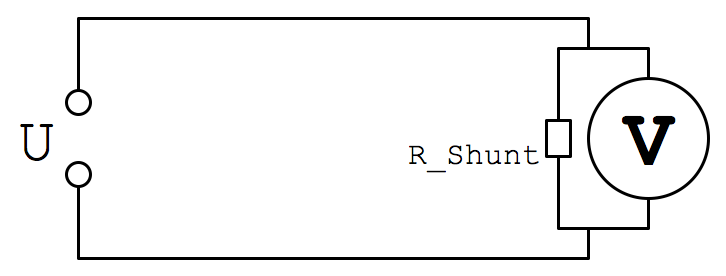
\includegraphics[width=\textwidth]{images/1a.png} %Schaltbild
\end{block}
\end{frame}
\section{Aufgabe 2}
\subsection{Tiefpass 1. Ordnung}
\begin{frame}
\begin{block}{Schaltplan des Filters}
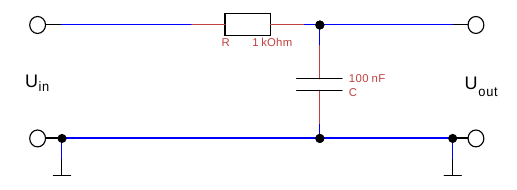
\includegraphics[width=\textwidth]{../daten/Messdaten/plots/schalt_tief}
\end{block}
\end{frame}
Bode-Diagramm:
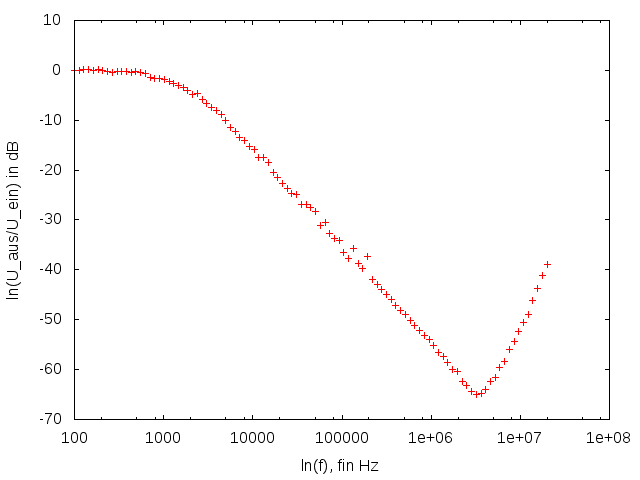
\includegraphics[width=\textwidth]{../daten/Messdaten/plots/Aufgabe2Bodediagramm_tief_gain}

Die "-3 dB-Frequenz" ist die Frequenz, bei der die ausgehende Spannung der Schaltung auf $\frac{U_{ein}}{\sqrt{2}}$ abgefallen ist. Diese Messung liefert $f_g = 1466.312710 Hz$.\\
Amplitude eines 

\subsection{Hochpass 1. Ordnung}
Schaltplan des Filters:\\

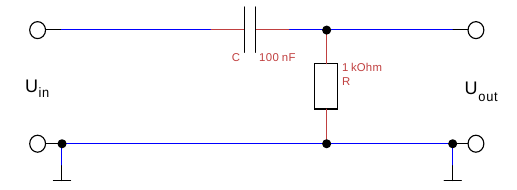
\includegraphics[width=\textwidth]{../daten/Messdaten/plots/schalt_hoch}
Bode-Diagramm:\\
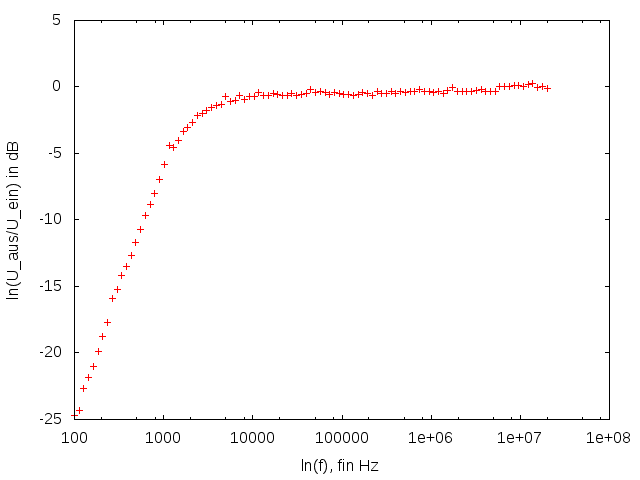
\includegraphics[width=\textwidth]{../daten/Messdaten/plots/Aufgabe2Bodediagramm_hochpass_gain}

$f_g \approx  1871.747229 Hz$

\subsection{AC-Modus des Oszilloskops}
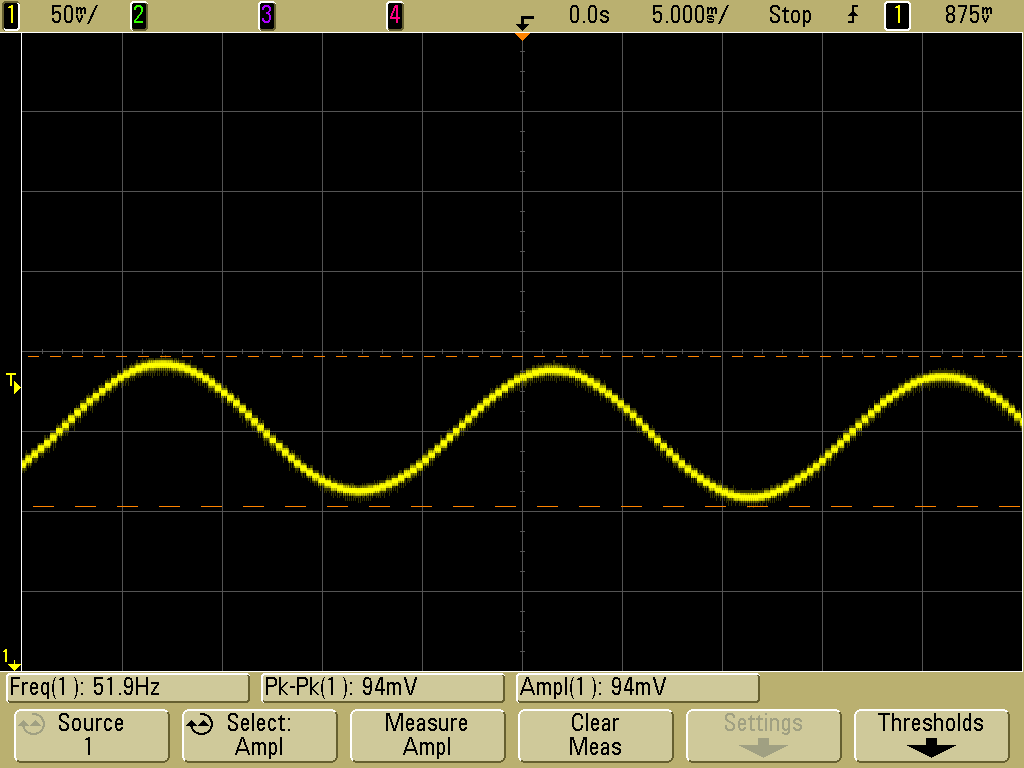
\includegraphics[width=\textwidth]{../daten/scope_16}
Signal trug zusätzlich zur Sinus-Schwingung noch eine Dreiecksspannung mit sehr niedriger Frequenz (der Verlauf deutet sich hier leicht an, da die Sinus-Welle leicht geneigt ist \\
Signal hat sich auf der Anzeige immer wieder leicht verschoben, es gab aber keine großen Probleme, es zu analysieren\\
$f_{sin} = 51.9 Hz$\\
$U_0 = 94 mV$

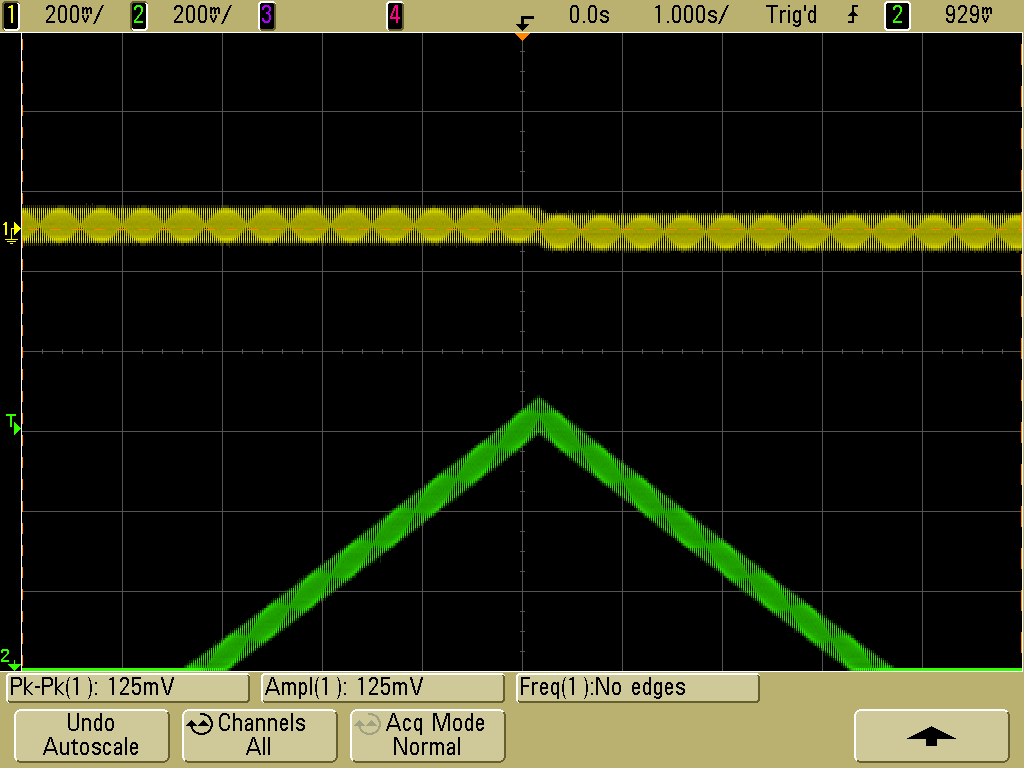
\includegraphics[width=\textwidth]{../daten/scope_21}
Vergleich zwischen Signal durch Hochpassfilter (gelb) und direkt in Oszilloskop (grün). Der Hochpass filtert die Dreiecksspannung aus dem Signal.

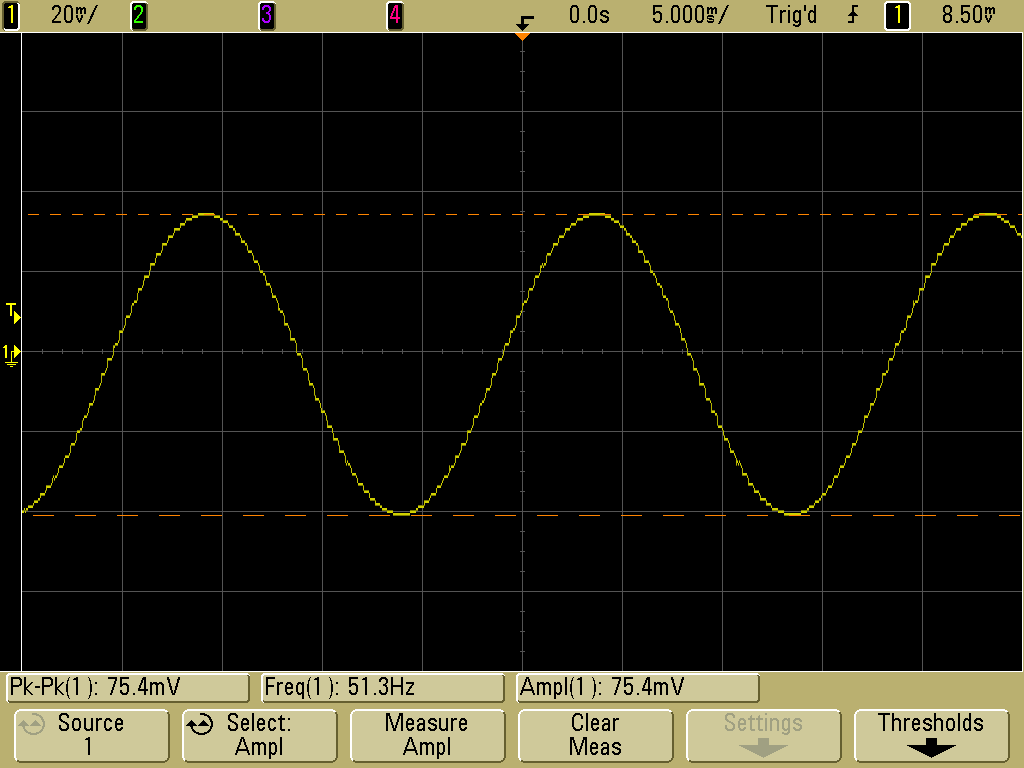
\includegraphics[width=\textwidth]{../daten/scope_22}

Mit dem AC-Modus aufgenommenes Signal\\
AC-Modus schaltet einen Hochpass-Filter zwischen Signal und Oszilloskop, der tieffrequente Schwingingen aus dem Signal entfernt
\section{Aufgabe 3}
\begin{frame}
\begin{block}{Gegebene Schaltung}
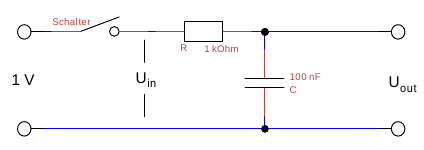
\includegraphics[width=\textwidth]{../daten/Messdaten/plots/schalt_tief2}
\end{block}
\end{frame}
\begin{frame}
Gemessene3 Sprungreaktion:\\
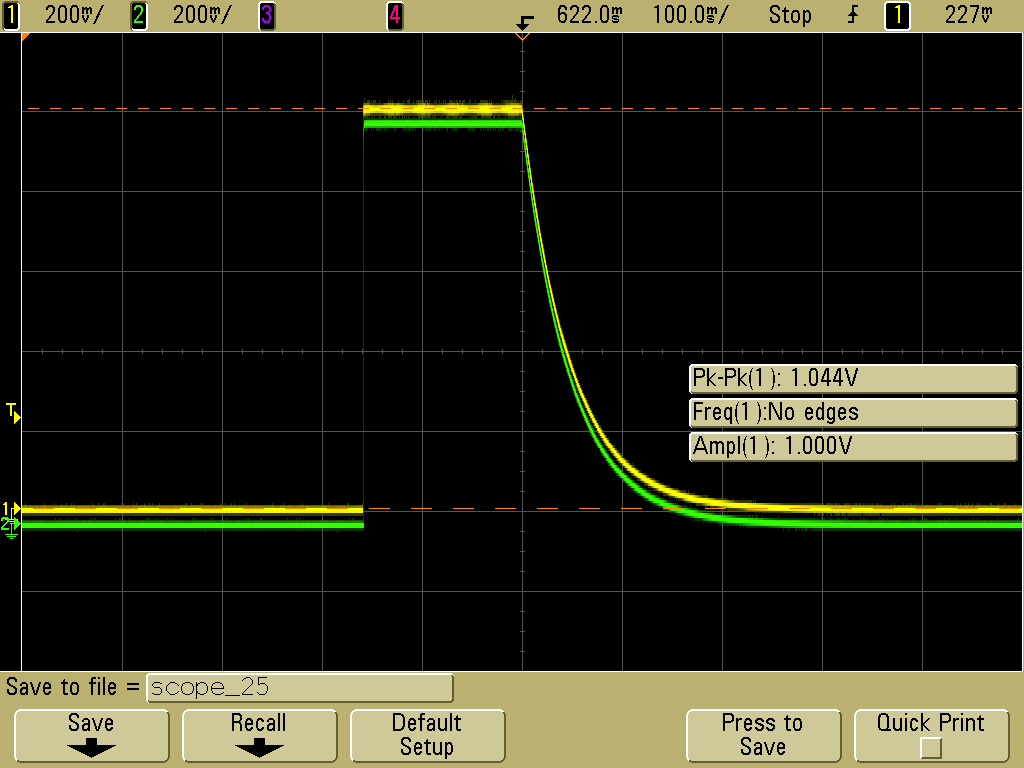
\includegraphics[width=\textwidth]{../daten/scope_25}
\end{frame}
\begin{frame}
Gesucht: Zeitkonstante $\tau = R \cdot C$\\
Sprungreaktion ist in diesem Fall der Entladevorgang des Kondensators, gegeben durch:
\begin{equation}
U(t) = U_0 * \exp(-\frac{t}{\tau}),  \tau = \frac{1}{R\cdot C}
\end{equation}
\end{frame}
\begin{frame}
Strategie: Setze $t=\tau$ $\Rightarrow  U(\tau) = U_0 \cdot \exp(-1)$\\
und suche den Wert $\frac{U(t)}{U_0} = \frac{1}{e}$ in der Messtabelle:
\begin{equation}
t \approx 0.045 s
\end{equation}
Errechneter Wert:
\begin{equation}
\tau = R \cdot C = 10^{-7} \cdot 10^{3} = 10^{-4}
\end{equation}
\end{frame}
\section{Aufgabe 4}
\begin{frame}
\begin{block}{Das fehlende Bauelement ist eine Drossel}
\centering
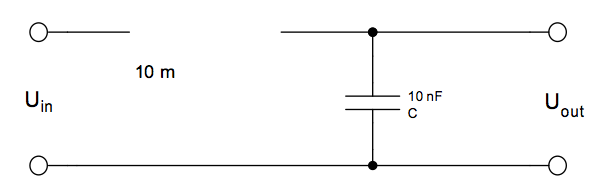
\includegraphics[width=\textwidth]{../daten/Messdaten/plots/schalt_4spule.png}
\end{block}
\end{frame}

\begin{frame}
\begin{block}{Messung mit Spule allein}
\centering
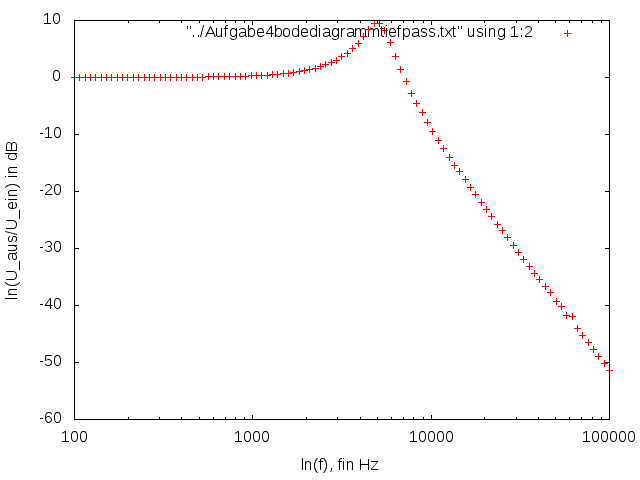
\includegraphics[width=.85\textwidth]{../daten/Messdaten/plots/Aufgabe4Bodediagramm_tief_gain}
\end{block}
\end{frame}

\begin{frame}
\begin{block}{Zweite Messung mit Widerstand in Reihe zur Spule}
\centering
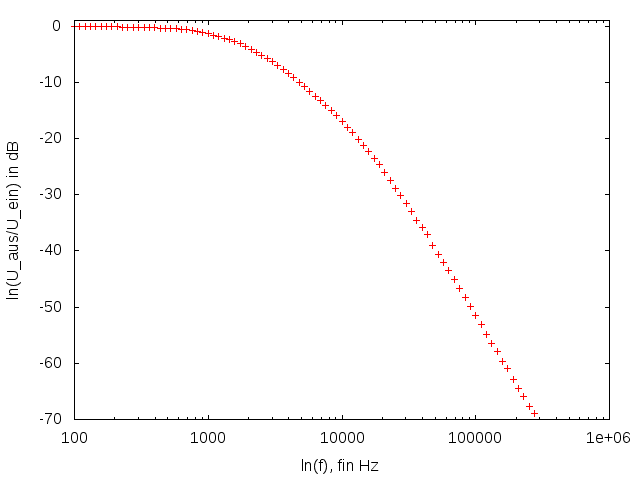
\includegraphics[width=0.85\textwidth]{../daten/Messdaten/plots/Aufgabe4Bodediagramm_tief_R_gain}
\end{block}
\end{frame}
\section{Aufgabe 5}
\subsection{a)}
\begin{frame}
\begin{block}{Zwei Peaks des Pulses}
\centering
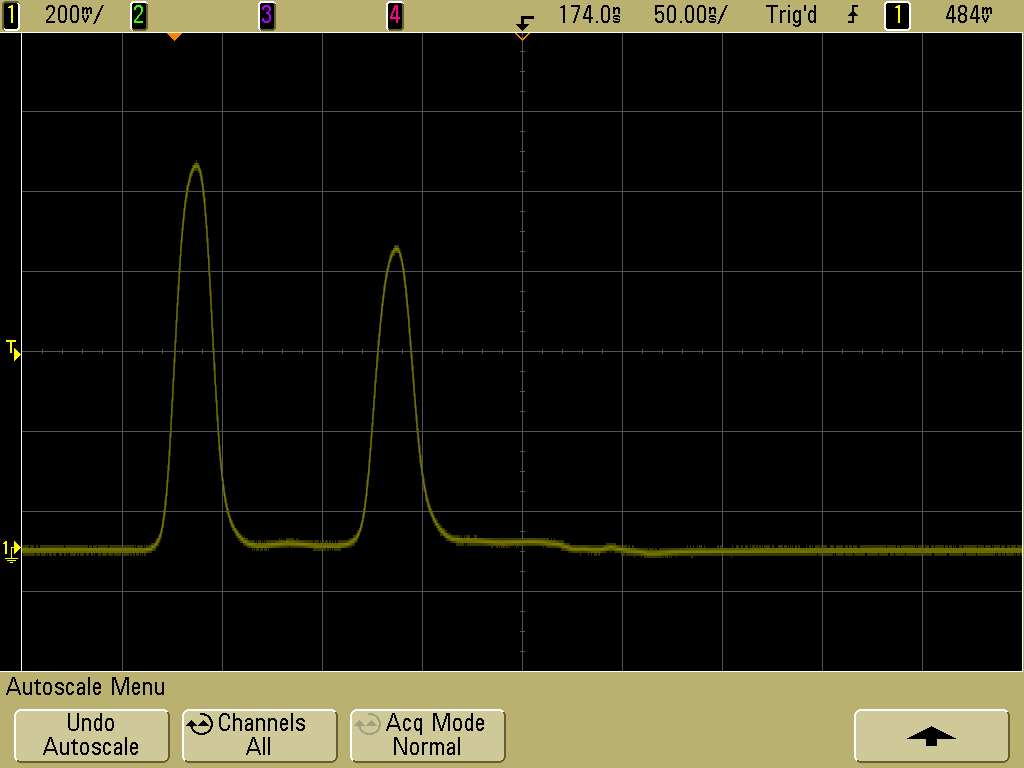
\includegraphics[width=.85\textwidth]{../daten/scope_28.png}
\end{block}
\end{frame}
\begin{frame}
\begin{block}{Zeitdifferenz zwischen den Peaks von $100 ns$}
\centering
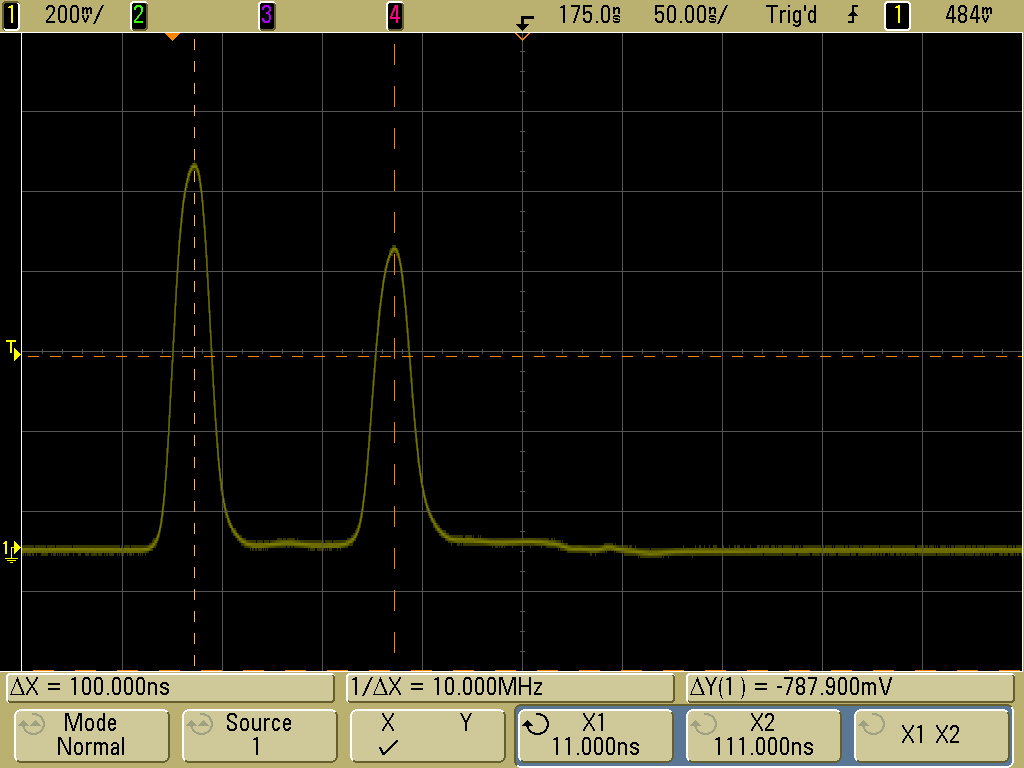
\includegraphics[width=.85\textwidth]{../daten/scope_29.png}
\end{block}
\end{frame}
\begin{frame}
Das Signal benötigt Zeit um sich im Kabel auszubreiten. Am offenen Ende des Kabels baut sich eine Spannung auf, die dazu führt, dass das Signal wieder in die Gegenrichtung fließt. \\
$\Rightarrow \Delta t$ ist die doppelte Laufzeit durch das Kabel
\end{frame}
\end{document}
